\documentclass[a4paper]{article}
\usepackage[utf8]{inputenc}
\usepackage[usenames,dvipsnames]{color}
% \usepackage{ngerman}
\usepackage{textcomp}
\usepackage{longtable}
\usepackage{amssymb}
\usepackage{helvet}
\usepackage{graphicx}
\usepackage{setspace}
\usepackage[super,square]{natbib}
\usepackage[colorlinks=true,linkcolor=black,citecolor=black,urlcolor=blue]{hyperref}
\usepackage[rflt]{floatflt}
\usepackage{geometry}
\usepackage{listings}
\usepackage{fancyhdr}
\geometry{a4paper,left=30mm,right=30mm,top=25mm,bottom=25mm}
% \renewcommand{\rmdefault}{\sfdefault}
\renewcommand{\headrulewidth}{0.0pt}

\newcommand{\cfile}[1]{\texttt{#1}}
\newcommand{\ccaption}[1]{\textsc{#1}}
\newcommand{\cvalue}[1]{\texttt{#1}}
\newcommand{\ckeyword}[1]{\texttt{#1}}

\newcommand{\note}[1]{\textbf{Note} #1 \par}
\newcommand{\warning}[1]{\textbf{Warning:} #1 \par}

\onehalfspacing

\lstset{
    basicstyle=\footnotesize\ttfamily, numbers=left, numberstyle=\footnotesize\ttfamily,
    keywordstyle=\color{blue}\bfseries, commentstyle=\color{Gray}\textit, stringstyle=\color{Maroon},
    stepnumber=1, numbersep=10pt, backgroundcolor=\color{white},
    frame=l, tabsize=2, captionpos=b, breaklines=true, breakatwhitespace=true,
    showspaces=false, showtabs=false, showstringspaces=false,
    title=\lstname, escapeinside={\%*}{*)},
    morekeywords={__file__}
}

\begin{document}

\pagestyle{fancy}
\fancyhf{}
\fancyfoot[R]{\huge{\thepage}}

\vspace*{\fill}
\begin{center}
  \Huge{\textbf{ORCF User Guide}} \\
  \vspace{2cm}
  \large{Written for ORCF \textbf{2011.07p}} \\
  \vspace{1cm}
  \large{\today}
  \vspace{3cm}
\end{center}
\vfill

\newpage

\tableofcontents

\newpage

\section{Getting started}
\subsection{What is ORCF?}
Open RollerCoaster Factory aims to be a free open-sorce theme park simulation game running on Linux, Mac OS X and Windows. Other than e.\,g.
Roller Coaster Tycoon, this is not about economy and money but about building and enjoying good-looking parks and extending the game with
custom objects and rides.

Although development started in November 2009, the game could not even reach its beta phase yet, but it is actively developed so that the first
stable version shall be released in September 2011.


\subsection{System requirements}
ORCF is a resource-hungry game relying on modern 3D technology and does therefore not run on every computer.

\subsubsection{Minimum}
\begin{itemize}
  \item Any x86 or x86\_64 CPU
  \item Video card with Shader Model 4.0 support (NVidia GeForce 8000 series or ATI Radeon HD 3000 series)
\end{itemize}

\subsubsection{Recommended}
\label{sysrecomm}
\begin{itemize}
  \item Dual-Core CPU with 2 GHz
  \item Very fast video card (NVidia GeForce 9800 GT, ATI Radeon HD 5450) with 512MB of dedicated VRam
  \item 2 GB of RAM
  \item A few GB of free HDD space for additional data packages
\end{itemize}


\subsection{Get ORCF}
At the moment there is no stable version of ORCF. There are development snapshots available as well as a continiously update GIT repository,
but all these sources have in common that they ship an unstable game that still lacks lot of features.

\subsubsection{Binary core packages}
Not available yet.

\subsubsection{Source core packages}
Not available yet.

\subsubsection{GIT version}
To clone the GIT repository, install GIT and do the following:
\begin{lstlisting}
$ git clone git://github.com/ireyon/Open-Rollercoaster-Factory.git orcf
\end{lstlisting}
Be warned: This contains the current development snapshot which is, in most cases, highly unstable and not ready for release.
If you want a working game, use the source or binary packages from above.

\subsubsection{Data packages}
In order to have something to build a park with, you need data packages you can find \dots nowhere yet.


\subsection{Compiling from source}
If you want to compile ORCF from source, which is needed when you downloaded the GIT version or a source package, you need at least Version
2.2 of the FreePascal compiler you can get either from your Linux distribution's package repositoríes or from the official
website\footnote{\url{http://www.freepascal.org/download.var}}.

\subsubsection{Linux}
You need to install OpenAL and SDL packages for ORCF to link properly. Development headers should not be needed.

Compile and start the game using the following commands:
\begin{lstlisting}
$ cd orcf
$ ./configure
$ make
$ make tools
$ ./orcf
\end{lstlisting}
There is currently no supported way of ``installing'' the game to \cfile{/usr/local}. Instead, you might move the entire ORCF directory to
\texttt{/opt} if you want multiple users to be able to use it.

\subsubsection{Mac OS X}
You need to install GLFW and OpenAL for ORCF to link properly.

Compile the game using the following commands:
\begin{lstlisting}
$ cd orcf
$ ./configure
$ make
$ make tools
$ ./bundle-orcf.sh
\end{lstlisting}
This should result in a working application bundle.

\subsubsection{Windows}
Compiling ORCF on Windows is somewhat trickier than on other systems. First, open \cfile{compile.bat} file in a text editor. You will see
three lines starting like
\begin{lstlisting}
fpc.exe -MObjFPC -g -Sghi -vewnhi  -Fu. -Fi. -Fu.\main 
\end{lstlisting}
Prepend the installation directory of your FreePascal compiler to every of these lines so that your computer can find it.

Now, run the compile.bat file either by double-clicking it from a file manager or from a CMD window. ORCF ships windows DLLs for SDL and
OpenAL so you don't need to install these.

If you used the GIT repository, create a directory named \cfile{config} in the orcf root directory before running the game.

\section{Settings}

When you first run the game, it will load some default settings: A 800 by 600 window, English language and poor graphics. If you want to
change it, click the \ccaption{Settings} button in the main menu.

\subsection{Language}
Currently there is only a text field where you can enter \cvalue{en} or \cvalue{de}, but there is no complete German translation yet.

You must restart the game for the changes to take effect.

\subsection{Screen}
Currently there are two text fields for the window dimensions.

You must restart the game for the changes to take effect.

\subsection{Graphics}

You can almost control everything related to rendering. The options are divided into the following four groups.

\subsubsection{General}
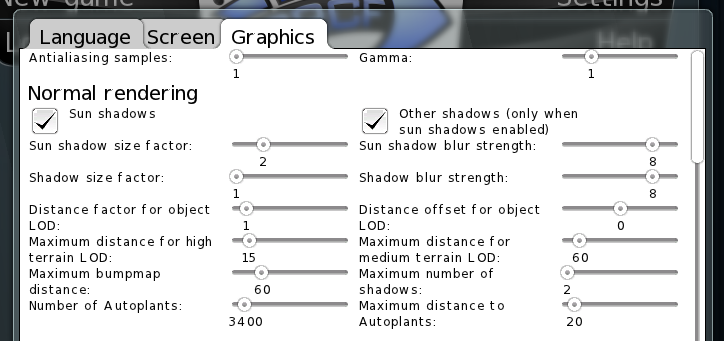
\includegraphics[width=140mm]{./images/settings-general.png}
\begin{description}
  \item[Antialiasing samples:] Specifies how many samples should be rendered per pixel. Higher values result in smoother edges, but
    also in significantly higher VRAM consumption and poor performance. Values of \cvalue{2} and more are good for videos.
  \item[Gamma:] Inverse exponent of each pixel. Does not affect user interface. Usually, \cvalue{1} is the best value.
  \item[Sun shadows:] When checked, the sun casts a shadow map.
  \item[Other shadows:] When checked, all light sources can cast shadows. However, it doesn't mean that every light source \emph{does}.
  \item[Sun shadow size factor:] Mulitplied by 1024, this value specifies the size of the sun shadow texture.
  \item[Shadow size factor:] Mulitplied by 256, this value specifies the size of the other shadow textures.
  \item[Sun shadow blur strength:] The blur radius for soft shadows casted by the sun. Higher values do \emph{not} mean stronger blur, but they \emph{do} mean nicer appearance of blurred shadows.
  \item[Shadow blur strength:] The blur radius for soft shadows casted by normal light sources.
  \item[Distance factor for Object LOD:] The minimum and maximum visibility ranges for objects will be multiplied by this value. The higher the value, the more details distant objects will have as long as they use LODs.
  \item[Distance offset for Object LOD:] Value to be added to visibility ranges. Normally, \cvalue{0} should do.
  \item[Maximum distance for high terrain LOD:] Size of the terrain quad containing the smallest sub blocks.
  \item[Maximum distance for medium terrain LOD:] Maximum distance for macro blocks with medium sized sub blocks.
  \item[Maximum bump map distance:] Distance to which the terrain appearance will be improved by normal maps.
  \item[Maximum number of shadows:] The number of normal light sources that will cast shadows. Only the light sources that affect the viewer's position most will get a shadow map.
  \item[Number of autoplants:] Number of quads that will be rendered for dynamic grass.
  \item[Maximum autoplant distance:] Distance after which auto plants will be removed and put elsewhere.
\end{description}

\subsubsection{Effects}
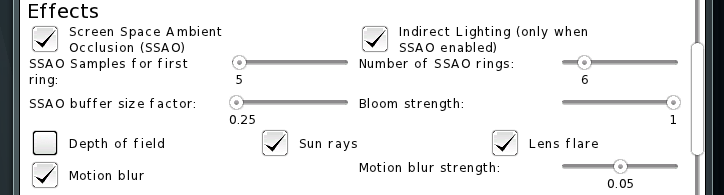
\includegraphics[width=140mm]{./images/settings-effects.png}
\begin{description}
  \item[Screen Space Ambient Occlusion (SSAO):] Effect that is used to gather details in shaded areas.
  \item[Indirect Lighting:] Effect that causes objects to be illuminated by light-emitting materials.
  \item[SSAO samples for first ring:] The number of pixels to be used for SSAO calculation in the first SSAO ring. If it is set to \cvalue{5}, it will use 10 samples for the second ring, 15 for the third and so on. The higher the value, the more accurate the effect will look.
  \item[Number of SSAO rings:] Number of SSAO rings. The higher the value, the more accurate the effect will look, but it has huge impact on overall performance.
  \item[SSAO buffer size factor:] Multiplied by the screen resolution, this will give the size of the SSAO buffer.
  \item[Bloom strength:] Strength of HDR bloom. Set to 0 or 1, anything else will look strange.
  \item[Depth of field:] When enabled, the object under the mouse cursor will be focussed, anything more or less distant will be blurred.
  \item[Sun rays:] Simulates visible sun rays that are especially nice on sunsets.
  \item[Lens flare:] Simulates camera lens effects.
  \item[Motion blur:] Moving parts of the scene will look a little blurry.
  \item[Motion blur strength:] The higher the value, the more blurry a moving scene will look.
\end{description}

\subsubsection{Water}
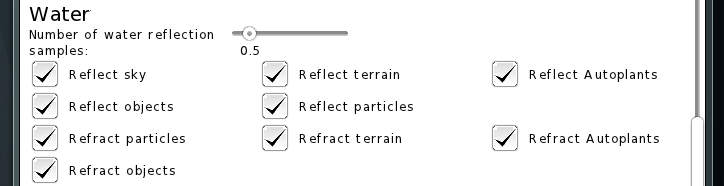
\includegraphics[width=140mm]{./images/settings-water.png}
\begin{description}
  \item[Number of water reflection samples:] Multiplied by the screen resolution, this represents the resolution of the water reflection and refraction buffers.
  \item[Reflect ...:] Speciefies what parts of the scene will be reflected in water.
  \item[Refract ...:] Speciefies what parts of the scene will be visible when looking from above into the water.
\end{description}

\subsubsection{Reflections}
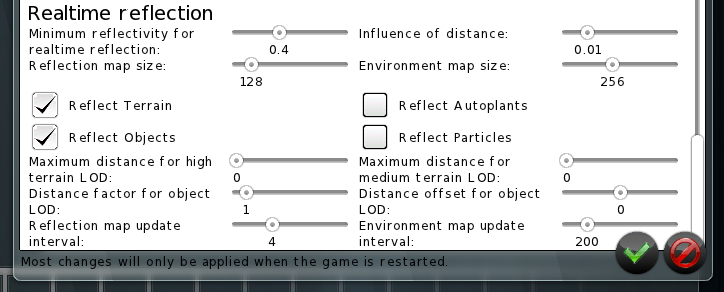
\includegraphics[width=140mm]{./images/settings-reflections.png}
\begin{description}
  \item[Minimum reflectivity:] Reflectivity value a material must have to be able to use realtime reflection.
  \item[Influence of distance:] The higher this is, the faster the minimum reflectivity value increases for distant objects. When too far away, even very reflective materials will only show the environment map to improve performance.
  \item[Reflection map size:] Edge length in pixels of the reflection maps.
  \item[Environment map size:] Edge length in pixels of the environment map.
  \item[Reflect ...:] Speciefies what parts of the scene shall be reflected in real time. The environment map only reflects the sky and the terrain.
  \item[LOD stuff:] See above.
  \item[Reflection map update interval:] Number of frames that shall pass before any of the dynamic reflection maps will be updated.
  \item[Environment map update interval:] Number of frames that shall pass before the static envionment map will be re-rendered.
\end{description}

\pagebreak[4]
\subsubsection{Presets}
Later, there will be some presets that makes the engine configuration much easier and faster.\nopagebreak

\begin{longtable}{|p{6cm}||c|c|c|c||c|}
\hline
 & Default & Performance & Quality & High Quality & Video \\ \nopagebreak
\hline
\hline
Sun shadows                    & & \checkmark & \checkmark & \checkmark & \checkmark \\ \nopagebreak
Other shadows                  & & & \checkmark & \checkmark & \checkmark \\ \nopagebreak
Sun shadow size factor         & & 2 & 2 & 2 & 3 \\ \nopagebreak
Shadow size  factor            & & & 1 & 2 & 2 \\ \nopagebreak
Sun shadow blur radius         & & 0 & 2 & 4 & 7 \\ \nopagebreak
Shadow blur radius             & & & 2 & 3 & 6 \\ \nopagebreak
Distance factor for objects    & 0.6 & 0.8 & 1 & 1.5 & 2 \\ \nopagebreak
Distance offset for objects    & 0 & 0 & 0 & 0 & 0 \\ \nopagebreak
High Terrain LOD distance      & 10 & 12 & 15 & 20 & 25 \\ \nopagebreak
Medium Terrain LOD distance    & 40 & 50 & 60 & 90 & 120 \\ \nopagebreak
Bumpmap Distance               & 40 & 50 & 60 & 90 & 120 \\ \nopagebreak
Number of shadows              & & & 5 & 10 & 20 \\ \nopagebreak
Number of autoplants           & 0 & 2000 & 3400 & 7700 & 13600 \\ \nopagebreak
Autoplant distance             & & 15 & 20 & 30 & 40 \\ \nopagebreak
\hline
\hline
Ambient Occlusion     & & & \checkmark & \checkmark & \checkmark \\ \nopagebreak
Indirect Lighting     & & & & \checkmark & \checkmark \\ \nopagebreak
SSAO Samples          & & & 5 & 7 & 9 \\ \nopagebreak
SSAO Rings            & & & 6 & 9 & 12 \\ \nopagebreak
SSAO buffer size      & & & 0.25 & 0.5 & 1.0 \\ \nopagebreak
Bloom strength        & 0 & 1 & 1 & 1 & 1 \\ \nopagebreak
Depth of field        & & & & \checkmark & \checkmark \\ \nopagebreak
Sun rays              & & & \checkmark & \checkmark & \checkmark \\ \nopagebreak
Lens flare            & & \checkmark & \checkmark & \checkmark & \checkmark \\ \nopagebreak
Motion blur           & & \checkmark & \checkmark & \checkmark & \checkmark \\ \nopagebreak
\hline
\hline
Reflection samples    & 0.25 & 0.33 & 0.5 & 0.75 & 1 \\ \nopagebreak
Reflect sky           & \checkmark & \checkmark & \checkmark & \checkmark & \checkmark \\ \nopagebreak
Reflect terrain       & & \checkmark & \checkmark & \checkmark & \checkmark \\ \nopagebreak
Reflect autoplants    & & & & \checkmark & \checkmark \\ \nopagebreak
Reflect objects       & & & \checkmark & \checkmark & \checkmark \\ \nopagebreak
Reflect particles     & & & & \checkmark & \checkmark \\ \nopagebreak
Refract terrain       & & \checkmark & \checkmark & \checkmark & \checkmark \\ \nopagebreak
Refract autoplants    & & & & \checkmark & \checkmark \\ \nopagebreak
Refract objects       & & & \checkmark & \checkmark & \checkmark \\ \nopagebreak
Refract particles     & & & & \checkmark & \checkmark \\ \nopagebreak
\hline
\hline
Minimum reflectivity             & 1.0 & 1.0 & 0.7 & 0.4 & 0.0 \\ \nopagebreak
Influence of distance            & & & 0.03 & 0.01 & 0.00 \\ \nopagebreak
Reflection map size              & & & 128 & 192 & 384 \\ \nopagebreak
Environment map size             & 128 & 192 & 256 & 384 & \\ \nopagebreak
Reflect terrain                  & \checkmark & \checkmark & \checkmark & \checkmark & \checkmark \\ \nopagebreak
Reflect objects                  & & & \checkmark & \checkmark & \checkmark \\ \nopagebreak
Reflect autoplants               & & & & & \checkmark \\ \nopagebreak
Reflect particles                & & & & & \checkmark \\ \nopagebreak
High terrain LOD distance        & & & 0 & 0 & 0 \\ \nopagebreak
Medium terrain LOD distance      & & & 0 & 0 & 25 \\ \nopagebreak
Distance factor for objects      & & & 1 & 1 & 2 \\ \nopagebreak
Distance offset for objects      & & & 0 & 0 & 0 \\ \nopagebreak
Reflection map update interval   & & & 4 & 2 & 1 \\ \nopagebreak
Environment map update interval  & 1000 & 500 & 200 & 100 & \\ \nopagebreak
\hline
\end{longtable}

\section{Gameplay}
At the moment, this is under heavy development. Although you can already modify the terrain and place simple objects, almost nothing
has the desired functionality yet.

\subsection{Terrain editing}
Due to the little block size, ORCF uses a marked area based terrain editor. Open it with a click on the terrain symbol and you will get
this window:

\begin{figure}[h]
  \begin{center}
    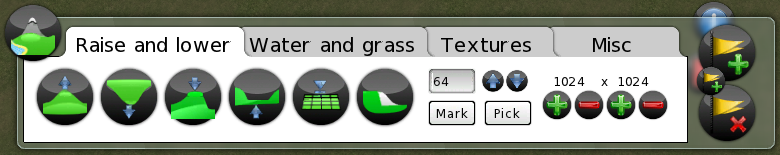
\includegraphics[width=140mm]{./images/terrain-01.png}
  \end{center}
  \caption{The terrain editor}
\end{figure}

\note{that the area \emph{not} belonging to your park will be darkened.}

\subsubsection{Creating marks}
The first step of every terrain editing action is to create a marked area. To add marks, click the large button with the \ccaption{add mark} icon.

\begin{figure}[h]
  \begin{center}
    
\includegraphics[width=10mm]{../images/selection-add.png}
    
\includegraphics[width=10mm]{../images/selection-delete.png}
  \end{center}
  \caption{The \ccaption{add mark} and \ccaption{remove mark} buttons}
\end{figure}

Now you can click on the terrain as much as you want to. Right-click an existing mark to delete it and left-click it to insert a new mark
after it. The currently placed mark appears in red color.

\note{that the larger the marked area is, the longer the terrain modifications will take. Creating a huge water layer sometimes takes up to
30 seconds in which the game seems to do nothing, although it is still running.}

\subsubsection{Selecting height}
The terrain editor has a text area with two arrows next to it. With that you can select the height level you want to raise a hill or cut
a valley to---but you can also pick the height level of the last mark you placed by pressing the \ccaption{Mark} button or select a height
level with the mouse by clicking \ccaption{Pick}.

\subsubsection{Modifying the landscape}
On the left of the terrain editor, you see six buttons. From left to right, these do the following:
\begin{itemize}
  \item 
\includegraphics[width=10mm]{../images/terrain-raise.png} creates a (kinda) smooth hill. Does not work perfectly yet on complex selections.
  \item 
\includegraphics[width=10mm]{../images/terrain-lower.png} creates a smooth valley with the same problems.
  \item 
\includegraphics[width=10mm]{../images/terrain-maximum.png} sets the maximum height of an existing hill.
  \item 
\includegraphics[width=10mm]{../images/terrain-minimum.png} sets the maximum height of an existing valley.
  \item 
\includegraphics[width=10mm]{../images/terrain-setfix.png} sets the height of the marked area exactly to the selected value.
  \item 
\includegraphics[width=10mm]{../images/terrain-smooth.png} tries to smooth the marked area. This is very slow.
\end{itemize}
\note{that objects that are placed in the modified area will \emph{not} be moved!}

\subsubsection{Resizing}
With the little 
\includegraphics[width=4mm]{../images/list-add.png} and 
\includegraphics[width=4mm]{../images/list-remove.png} you can resize
the terrain along the X and Z axes. The larger your building area is, the more you can do, but the slower further modifications will be. The
file size of a stored park will also increase by a lot.
\note{that the numbers (1024, ..) are the number of sub blocks in either direction, not meters. If you want meters, divide it by 5.}
\note{that the default building area is quite small. It has only 204.8x204.8 meters, whereas an empty park in RCT3 has something like
512x512 meters.}
\note{that a feature to move the entire park along the axes is planned, but not implemented yet.}

\subsubsection{Water}

\begin{figure}[h]
  \begin{center}
    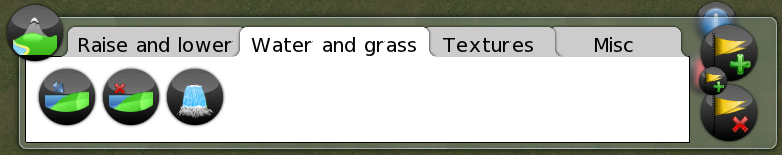
\includegraphics[width=140mm]{./images/terrain-02.png}
  \end{center}
  \caption{The water and grass tab}
\end{figure}

Water is one of the best-working features, although stuff like waterfalls is still missing. To create a new water surface,
click the \ccaption{Set water} button. You will get a height line under which the water will be. However this doesn't set the water level for the
entire park, it rather fills the connected region under your mouse. So, if you want to fill a region and the height line is interrupted,
only a smaller part will be filled.
\note{that this again is very, very slow.}

If you want to delete a water surface, click the \ccaption{Delete water} button and select a surface. No height lines here.

\begin{figure}[h]
  \begin{center}
    
\includegraphics[width=10mm]{../images/terrain-setwater.png}
    
\includegraphics[width=10mm]{../images/terrain-deletewater.png}
  \end{center}
  \caption{\ccaption{Set water} and \ccaption{Delete water}}
\end{figure}

\subsubsection{Changing textures}

\begin{figure}[h]
  \begin{center}
    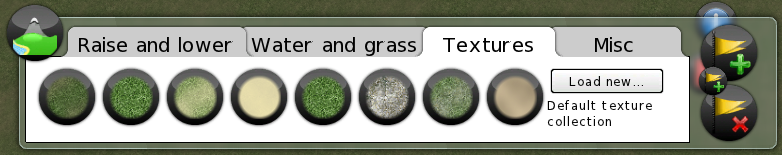
\includegraphics[width=140mm]{./images/terrain-03.png}
  \end{center}
  \caption{Everything about the terrain texture collection}
\end{figure}

If you want an area to look sandy, dirty, rocky or snowy, you can choose between eight textures supplied by a so-called texture collection.
Click on one of the eight round buttons and the area you marked will be changed. This is usually relatively fast.

\subsubsection{Changing the texture collection}
If you don't like the default eight textures, you can load other terrain texture collections with the \ccaption{Load new} button.
It will also replace the autoplant appearance.

\subsubsection{Other stuff}

\begin{figure}[h]
  \begin{center}
    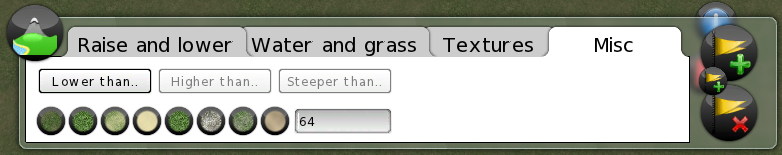
\includegraphics[width=140mm]{./images/terrain-04.png}
  \end{center}
  \caption{Some other functions}
\end{figure}

The left part is used for conditional texture changes. If you, let's say, have a mountain and you only want the top of it look like snow,
you can enter the height level you like in the text area (or just pick it with the functions in the \ccaption{Raise and Lower} tab),
the select \ccaption{Higher than\dots} and the desired snow texture.
\note{that for \ccaption{Steeper than\dots}, the compared values are usually somewhere between 0 and 2. No picking here (yet), sorry.}

\subsection{Building objects}
In ORCF, you are almost free where and how to place objects. The only limitations are the building area of the park, the accuracy of
32 bit floating point numbers and a height of about 250 meters.

\subsubsection{Selecting the object to build...}
All objects, rides and pathes can be built using the object selector. Click on the \ccaption{Objects} button.
\begin{figure}[h]
  \begin{center}
    
\includegraphics[width=10mm]{../images/park-objects.png}
  \end{center}
  \caption{The \ccaption{Objects} button}
\end{figure}

You will get a large window looking like this:
\begin{figure}[h]
  \begin{center}
    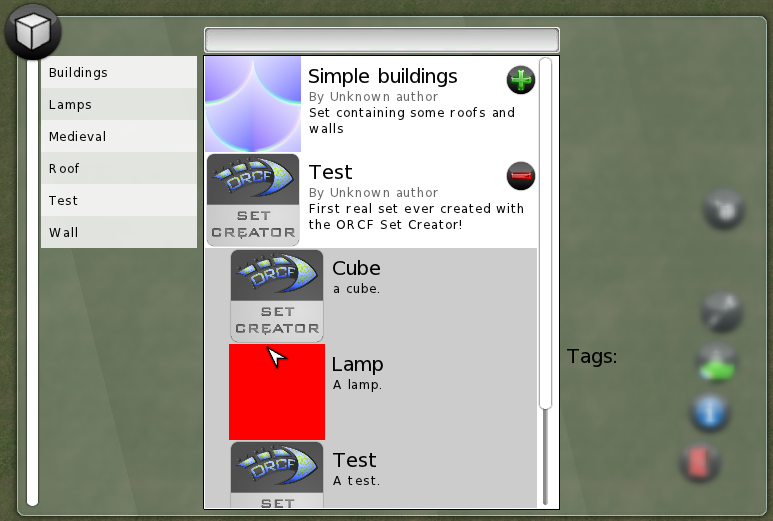
\includegraphics[width=140mm]{./images/objectselector.png}
  \end{center}
  \caption{The object selector}
\end{figure}

On the left part, you can select or deselect groups. Objects that are in any of the selected groups will be shown in the middle park.
So, if you only want medieval lamps, I have to disappoint you, you will most probably have to search them in the list of lamps or in
the list of medieval objects.

The search bar on the top of the window behaves differently, only objects and sets that match every word in their name, their author's name
or their description.

Once you select an object from the middle part, metadata such as groups the object belongs to will be displayed. A big \ccaption{Add}
button will appear in the bottom right corner when the object is loaded---that might take a while, especially scripted objects might take a
second more to get ready.

\subsubsection{Placing an object}
When you click that button, the object builder window will open:
\begin{figure}[h]
  \begin{center}
    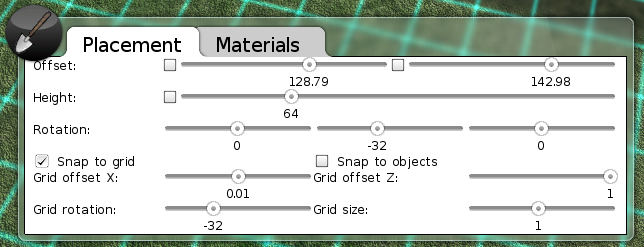
\includegraphics[width=120mm]{./images/objectbuilder.png}
  \end{center}
  \caption{The object builder}
\end{figure}

That's a lot of sliders, I agree. But you don't need to change any of them normally: If you move the mouse over the park, you'll see that the
object adjusts to your mouse position and the \ccaption{Position} and \ccaption{Height} sliders change as well.

If you want to lock any of the position axes, tick the check box next to the sliders. They won't change anymore.

If you press \ccaption{Ctrl} and scroll your vertical mouse wheel, the object will go up and down, the Y position (\ccaption{Height}) will
be locked.

If you press \ccaption{Ctrl} and your middle mouse button and move the mouse to the left or right, you rotate the object in 5 degree
steps along the Y axis. To rotate around the other axes, you must adjust the sliders.

When the grid is enabled, you might want to rotate it the same way as the object. To do that, press \ccaption{Ctrl} and your right mouse
button, you can rotate the grid just like the object.

Play around with the other otions to see what they do.

\subsubsection{Coloring an object}
There is this nice \ccaption{Material} tab in the object builder. When you click that, you will see a list of materials on the left and the
properties of the currently selected material on the right. You can change the color, the level of light emission and the reflectivity
of every material. The names of the materials are stored in the objects themselves, which makes the object's author responsible for them.

\begin{figure}[h]
  \begin{center}
    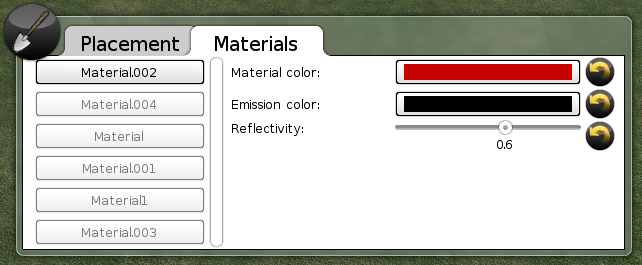
\includegraphics[width=120mm]{./images/objectmaterials.png}
  \end{center}
  \caption{The material editor}
\end{figure}

If you accidentally changed something you didn't want to change, just click the \ccaption{Revert} button next to the property you want to
reset.
\begin{figure}[h]
  \begin{center}
    
\includegraphics[width=10mm]{../images/edit-undo.png}
  \end{center}
  \caption{The \ccaption{Revert} button}
\end{figure}

\subsubsection{Modifying built objects}
Under normal circumstances, you only have to click on an object to edit its materials or to move it around.

\subsubsection{Deleting objects}
To delete an object, you first of all have to change the selection mode.
\begin{figure}[h]
  \begin{center}
    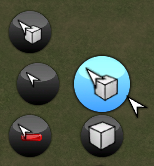
\includegraphics[width=30mm]{../images/selectionmodes.png}
    
\includegraphics[width=10mm]{../images/selection-default.png}
    
\includegraphics[width=10mm]{../images/selection-none.png}
    
\includegraphics[width=10mm]{../images/selection-remove.png}
  \end{center}
  \caption{Three selection modes: \ccaption{Normal}, \ccaption{Disabled} and \ccaption{Delete}.}
\end{figure}
Click the \ccaption{Delete} button and then select the object you want to delete. \note{that the game does not ask you whether you really
want to remove an object or not. Be careful with transparent objects as well.}

You can also use the keys \ccaption{1}, \ccaption{2}, \ccaption{3} on your keyboard (not on the numblock!) to change the selection mode. Don't
forget to reset it when you don't want to delete anything anymore.

\subsection{Building pathes}
Not implemented yet. Will be something using Bézier curves.

\subsection{Building flatrides}
Not implemented yet. Will almost be the same as objects.

\subsection{Building tracked rides}
Not implemented yet. Again, something like objects with Bézier curves.

\subsection{Taking screenshots}
When you press \ccaption{F10}, a screenshot will be recorded and saved in the screenshots directory somewhere in the ORCF home data path.
When pressing \ccaption{Ctrl+F10}, the user interface will be included in the screenshot.

\subsection{Recording videos}
When you press \ccaption{F11}, a video will be recorded and saved in the screenshots directory somewhere in the ORCF home data path.
When pressing \ccaption{Ctrl+F11}, the user interface will be included in the video.

ORCF stores every single frame as a TGA file. Therefore you must encode it to a format your favorite video editing software can handle. This
can be done for example using ffmpeg\footnote{\url{http://www.ffmpeg.org/download.html}}. If you prefer applications with a graphical user
interface, I still have to disappoint you, but ORCF will get an interface for ffmpeg later. But that's something for a stable version.

\subsubsection{Encoding with ffmpeg}
ffmpeg is a cross-platform command line utility with which you can transcode video and audio between a vast number of codecs and container
formats and even has the ability to read input from single images like TGA files.

To encode a video, do the following:
\begin{lstlisting}
$ cd ~/orcf-data/Videos/Video_0
$ ffmpeg -r 25 -i frame_08d.tga -vcodec libtheora -vb 8000k video.ogg
\end{lstlisting}

\note{that not every video editing software can handle OGG/Theora video. Replace \cvalue{libtheora} by \cvalue{libx264} or \cvalue{mpeg4} and
\cvalue{video.ogg} by \cvalue{video.avi}, \cvalue{video.mp4} or \cvalue{video.mkv} in order to get more compatible files.}
\note{that you must use \textbackslash{} instead / of on Windows.}
\note{that the bitrate of \cvalue{8000k} is good for 1280x720 videos. Increase it to \cvalue{16000k} for 1920x1080 and use lower bitrates
for lower resolutions}

\subsection{Creating cameras and camera routes}
Not implemented yet.

\subsection{Saving a park}
Click on the quit icon and then save the park file using the save button.
\begin{figure}[h]
  \begin{center}
    
\includegraphics[width=10mm]{../images/leave.png}
    
\includegraphics[width=10mm]{../images/document-save-as.png}
  \end{center}
  \caption{The quit and save icons.}
\end{figure}

\section{Troubleshooting}
If you have problems, make sure that:
\begin{itemize}
  \item your computer matches the recommended system specifications as listed in \ref{sysrecomm}
  \item you use the latest official ORCF release
  \item you did not mess up your ORCF install by violently deleting or moving important files or directories.
\end{itemize}

To report a bug, contact me via mail, ICQ, XMPP, whatever way you like, describe the problem as good as possible and also tell me what kind
of data files you used before the game crashed or behaved an unexpected way. In some cases it might be needed to attach the park file as well,
bugs can only be fixed when the developer can reproduce them.

\end{document}